\chapter{\Large Iteración I: “Despliegue e instalación de Security Onion en un ambiente de prueba”}
    En este capítulo describimos la instalación de Security Onion en la topología de red de prueba. Se instalará un nodo \textit{Master}, dos nodos \textit{Forward} y un nodo de \textit{TheHive}. \par
    En este proyecto se trabajó primero sobre un ambiente de prueba y después de producción. En ambos casos se utilizó un servidor central y un sistema operativo de virtualización sobre el que se crearon un conjunto de máquinas virtuales, cada una alojando un servidor con nodos \textit{Forward}, \textit{Master} y el correspondiente a TheHive - Cortex. Se utilizó de guía los componentes, el software y la arquitectura de conexión entre ellos, mencionados en la Descripción de Security Onion. \par
    \begin{section}{Topología de la organización}
    El paso inicial consistió en relevar la topología de la organización, para ello se dispuso de información inicial que fue brindada por los responsables del sector de redes. Posteriormente se realizaron diagramas topológicos con el fin de evaluar la situación y contemplar distintas estrategias para el despliegue de este proyecto.  
    En la Figura \ref{fig:iter1_top_unc} se observa un diagrama que representa la topología de la organización.\par
    Se puede apreciar que las dependencias están conectadas (mediante sus \textit{routers} de borde) entre sí y al mundo exterior mediante el Switch 1 de capa 3 que se encuentra en el \textit{datacenter}. Se observan los servidores 1, 2 y N que representan los activos de información de la organización, éstos están conectados mediante el \textit{Switch} 2 al resto de la organización. Existen M \textit{switches} para otras redes internas del \textit{datacenter}, todos conectados al \textit{Switch} 2. Este \textit{switch}, por lo tanto, conecta las redes internas del \textit{datacenter} y los activos de información con el \textit{Switch} 3, siendo este último el \textit{switch} troncal de la organización. Los enlaces anteriormente mencionados, incluidos los que conectan los \textit{routers} de borde de las dependencias y el \textit{Switch} 3, poseen un ancho de banda de 1 Gbps.\par
    Se observan otros componentes de la infraestructura de la organización, encargados de la conexión exterior con el resto del mundo. Estos son el \textit{Firewall} entre el \textit{Switch} 1 y el \textit{Switch} 5, los \textit{Routers} de borde 1 y 2 junto al \textit{Switch} 6 que se conecta a los proveedores ISP. Todos los enlaces entre estos componentes tienen como característica común un ancho de banda de 10 Gbps. \par
    \begin{figure}[H]
    \centering
    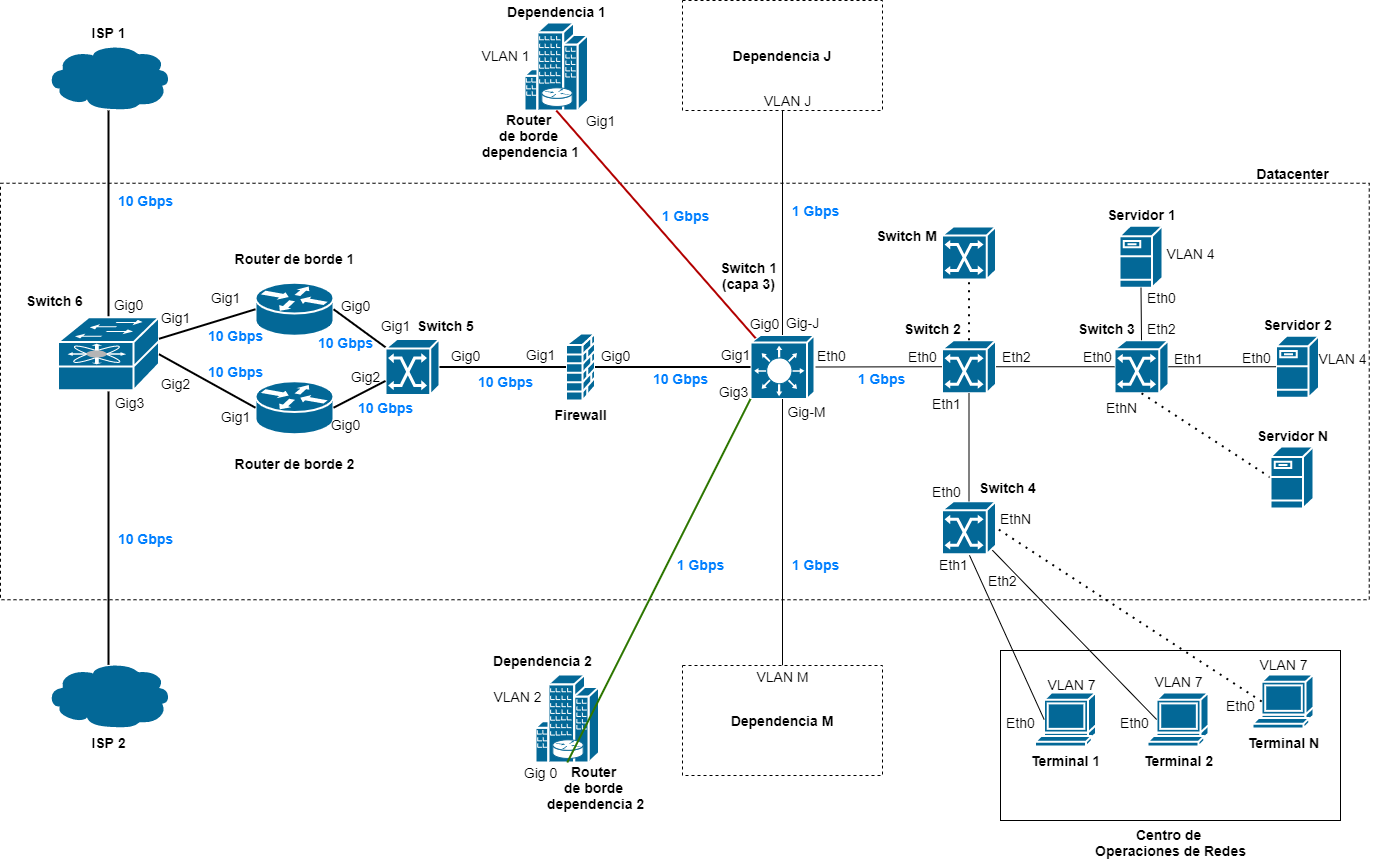
\includegraphics[width=1\textwidth]{./iteracion_1_imagenes/figura_topologia_UNC.png}
    \caption{Topología de la Organización}
    \label{fig:iter1_top_unc}
    \end{figure}
    \FloatBarrier
    \end{section}
    \begin{subsection}{Definición y configuración de las redes a observar}
    Se analizó el ancho de banda de las dependencias existentes y se decidió monitorear dos de ellas. Se seleccionaron las de mayor volumen de tráfico en función de mediciones realizadas a lo largo de una semana y de datos históricos. Las dependencias seleccionadas tenían un enlace con ancho de banda de 1 Gbps cada una. \par
    Las Figuras \ref{fig:figura_35_trafico_dia} muestra el volumen de tráfico medido en un periodo de tiempo de un día (exceptuando las horas en las que la actividad era mínima), mientras que en la Figura \ref{fig:figura_36_trafico_semana} muestra un periodo de una semana. Estos gráficos fueron obtenidos mediante el uso de LibreNMS \cite{librenms} (versión 1.48).\par
    Los datos de las Figuras 5.2 y 5.3 fueron tomados desde la interfaz Gig0 del \textit{Switch} 1 de la Figura 5.1, esto quiere decir que el volumen de tráfico corresponde a la Dependencia 1. Las interfaces Gig3, Gig-M y Gig-J del \textit{Switch} 1 tenían un comportamiento similar.\par
    \begin{figure}[H]
    \centering
    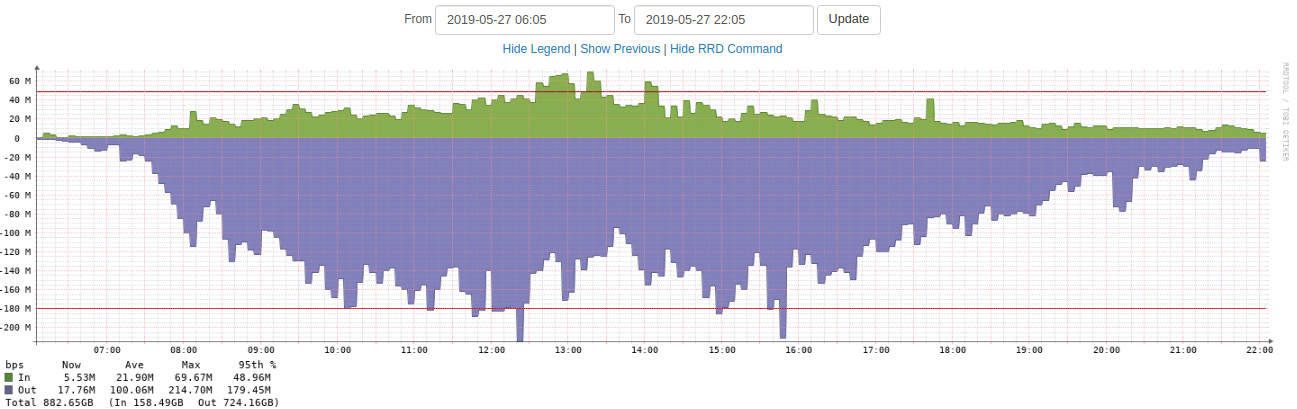
\includegraphics[width=1\textwidth]{./iteracion_1_imagenes/figura_35_trafico_dia.png}
    \caption{Tráfico correspondiente a una dependencia, medido durante un día }
    \label{fig:figura_35_trafico_dia}
    \end{figure}
    \begin{figure}[H]
    \centering
    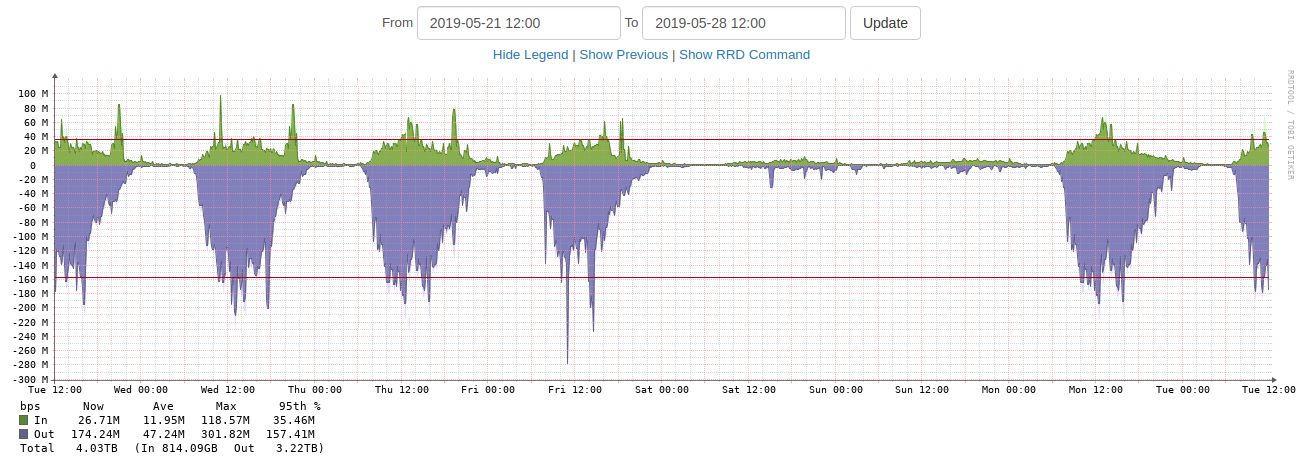
\includegraphics[width=1\textwidth]{./iteracion_1_imagenes/figura_36_trafico_semana_editada.png}
    \caption{Tráfico medido durante el periodo correspondiente a una semana}
    \label{fig:figura_36_trafico_semana}
    \end{figure}
    \FloatBarrier
    En la Figura 5.3 se observa el tráfico de la interfaz Gig0 en el periodo de una semana, donde la velocidad promedio correspondiente a la entrada es de 11,95 Mbps, mientras que de salida es de 47,24 Mbps. Se observaron picos de 300 Mbps de tráfico.\par
    Como la medición corresponde a la interfaz Gig0, el tráfico entrante a esta corresponde al de subida de la Dependencia 1, mientras que el tráfico saliente corresponde al de bajada de esta dependencia.
    \end{subsection}
    \begin{subsection}{Selección de hardware}
    \label{seleccion_hw}
    En primer lugar se examinaron los requisitos de hardware mínimos y recomendados por cada uno de los fabricantes. Para esto se tuvo en cuenta el ancho de banda y el tráfico de los enlaces a monitorear, descritos en la sección precedente. Los requerimientos se presentan a continuación, en los Cuadros \ref{table:15} y \ref{table:5} (para nodos Monolítico y Distribuido, respectivamente). \par
    En base a la Figura \ref{fig:iter1_top_unc}, los datos referidos al tráfico y el ancho de banda de los enlaces a monitorear, se dimensionó el hardware necesario para el servidor central, teniendo en cuenta los requerimientos del fabricante y las limitaciones disponibles en la organización.\par
    %Tabla HW nodo Monolitico
    \begin{table}[H]
    \centering
    \begin{tabular}{|m{10em}|m{10em}|}
    \hline 
    Requerimiento  & Nodo Standalone \\ 
    \hline
    Cantidad de CPU - Arquitectura &  10 nucleos vCPU - x86-64  \\ \hline
    Memoria RAM  &  32 GB  \\ 
    \hline
    Almacenamiento necesario   & 200 GB  \\
    \hline
    Cantidad de interfaces de red  & 2 (administración y monitoreo) \\
    \hline %linea final de tabla
    \end{tabular}
    \caption{Requerimientos de hardware para un nodo Standalone, según el fabricante.}
    \label{table:15}
    \end{table}
     %Tabla HW topología distribuida  
    \begin{table}[H]
    \centering
    \begin{tabular}{|m{9em}|m{9em}|m{9em}|m{9em}|}
    \hline 
    Requerimiento  & Nodo \textit{Master} &  Nodo \textit{Forward} & TheHive y Cortex \\ 
    \hline
    Cantidad de CPU - Arquitectura & Mínimo de 8 núcleos vCPU - x86-64 & Mínimo de 12 núcleos vCPU - x86-64 & Mínimo de 8 núcleos vCPU - x86-64 \\ 
    \hline
    Memoria RAM  & 12 a 128 GB & 128 a 256 GB & A partir de 8 GB \\ 
    \hline
    Almacenamiento necesario & Mínimo de 1 TB  & Mínimo de 540 GB & A partir de 60 GB \\
    \hline
    Cantidad de interfaces de red & 1 (administración) & 2 (administración y monitoreo) & 1 (administración) \\
    \hline %linea final de tabla
    \end{tabular}
    \caption{Requerimientos de hardware recomendados por el fabricante para el monitoreo de un enlace de 1 Gbps}
    \label{table:5}
    \end{table}
    Debido a las restricciones en la disponibilidad del hardware, se realizó una implementación aproximada, teniendo en cuenta los recursos disponibles en la organización. A continuación se muestran los recursos de hardware utilizados, según se trate del despliegue de una topología Monolítica (Cuadro \ref{table:16}) o de una Distribuida (Cuadro \ref{table:12}). \par
    \begin{table}[H]
    \centering
    \begin{tabular}{|m{10em}|m{10em}|}
    \hline 
    Requerimiento  & Nodo Standalone \\ 
    \hline
    Cantidad de CPU - Arquitectura &  4 núcleos vCPU - x86-64  \\ 
    \hline
    Memoria RAM  &  16 GB  \\ 
    \hline
    Almacenamiento necesario   & 500 GB  \\
    \hline
    Cantidad de interfaces de red  & 2 (administración y monitoreo) \\
    \hline %linea final de tabla
    \end{tabular}
    \caption{Requerimientos de hardware utilizados para el despliegue del nodo Standalone.}
    \label{table:16}
   \end{table}
    %En el caso de la topología Distribuida, el hardware que se utilizó para cada nodo se muestra en el Cuadro \ref{table:12}.
    \begin{table}[H]
    \centering
    \begin{tabular}{|m{9em}|m{9em}|m{9em}|m{9em}|}
    \hline 
    Requerimiento  & Nodo \textit{Master} &  Nodo \textit{Forward} & TheHive y Cortex \\ 
    \hline
     Cantidad de CPU - Arquitectura & 8 nucleos vCPU - x86-64 & 10 nucleos vCPU - x86-64 & 8 nucleos vCPU - x86-64 \\ 
    \hline
    Memoria RAM  & 16 GB & 32 GB & 8 GB \\ 
    \hline
    Almacenamiento necesario & 500 GB  & 200 GB & 60 GB \\
    \hline
    Cantidad de interfaces de red & 1 (administración) & 2 (administración y monitoreo) & 1 (administración) \\
    \hline %linea final de tabla
    \end{tabular}
    \caption{Requerimientos de hardware utilizado según el tipo de nodo desplegado.}
    \label{table:12}
    \end{table}
    \end{subsection}
    \pagebreak
    \begin{subsubsection}{Características del hardware empleado}
    Se dispuso de varios servidores centrales en los cuales se albergaron las máquinas virtuales de este proyecto. Si bien cada uno de ellos contaba con distinta capacidad de hardware, estas diferencias eran sólo cuantitativas, ya que las características del hardware para todos los servidores eran las mismas. A continuación, se detallan las más relevantes:
   \begin{itemize}
    \item En cuanto a los núcleos de CPU virtuales, su frecuencia era de 2.4 Ghz, basados en procesadores físicos Intel Xeon E5620.
    \item Las memorias RAM pertenecían a la tecnología DDR3 y su frecuencia de refresco era de 2400 MHz.
    \item Los discos utilizados fueron del tipo mecánico con una velocidad de transferencia para lectura de 196 MB/s y para escritura de 154 MB/s, con interfaz SATA III y 7200 rpm de velocidad de rotación.
    \end{itemize}
    \end{subsubsection}
    
    \begin{subsection}{Pérdidas de paquetes}
    Como consecuencia de no satisfacer los requerimientos de hardware recomendados por el fabricante, para los nodos que contienen sistemas IDS, se detectó una pérdida de paquetes que varía según el volumen de tráfico. El estudio de este problema fue realizado por otro grupo, que llevó a cabo su Proyecto Integrador sobre sistemas IDS. Se realizaron pruebas con diferentes velocidades de tráfico y se observo un porcentaje de paquetes que se perdía dependiendo de la velocidad del enlace, como se aprecia en el Cuadro \ref{table_13}.\par
    \begin{table}[H]
    %\centering
    \resizebox{\textwidth}{!}{
    \begin{tabular}{|c|c|c|} 
    \hline
    Velocidad (Mbps) &  Pérdidas de paquetes (\%) & Alertas sin detectar (\%)\\
    \hline
    800 & 25 & 40 \\
    \hline
    400 & 12 & 20 \\
    \hline
    200 & 0 & 0 \\
    \hline %linea final de la tabla
    \end{tabular}
    }
    \caption{Perdida de paquetes y alertas no detectadas, según la velocidad del enlace}
    \label{table_13}
    \end{table}
    La pérdida de paquetes por parte de los IDS tuvo como consecuencia una disminución en la cantidad de alertas detectadas. En base a pruebas llevadas a cabo con TCPreplay\cite{tcpreplay} enviando PCAPs con ataques a los sistemas IDS, con duración de un día cada prueba, se estimó el porcentaje de alertas sin detectar según el porcentaje de pérdidas de paquetes. Los resultados de estas pruebas se observan en el Cuadro \ref{table_13}.
    \end{subsection}
    \begin{section}{Monitoreo de red}
    A pesar de conocer, por la sección anterior, que el rendimiento de una topología monolítica no es óptimo en entornos de alto rendimiento, se decidió desplegar esta topología en primer lugar para familiarizarnos con la solución.\par
    \end{section}
    \begin{subsection}{Topología Monolítica de Monitoreo}
    \label{subsec-topo-mono}
    En la Figura \ref{fig:figura_33_a}, se observa una topología de prueba desarrollada en una red aislada, a modo de experiencia de laboratorio, en el cual se desplegó la solución con una arquitectura monolítica.\par
    El experimento consistió en demostrar la capacidad de monitoreo y detección de incidentes de Security Onion, mediante el despliegue de un nodo Monolítico y tres terminales de computadoras, una de las cuales (C) simuló ser el atacante.\par
    En primer lugar, se conectaron las terminales “A” y “B” (la del analista y el generador de logs, respectivamente) a un switch al cual se conectó, mediante su interfaz “Eth1”, uno de los enlaces del servidor de Security Onion. Este enlace, llamado “Eth0” en la Figura \ref{fig:figura_33_a}, sirvió a fines de que el analista en el terminal “A” simule consultas y visualice datos en Security Onion, mientras que el terminal “B” envíaba logs mediante Filebeat \cite{filebeat}, conteniendo información contextual de los activos de la red. \par
    \begin{figure}[H]
    \centering
    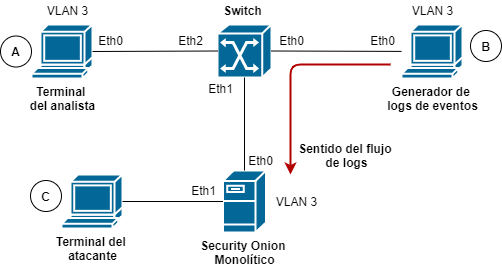
\includegraphics[width=0.8\textwidth]{./iteracion_1_imagenes/figura_33_a_topologia_de_prueba_1.png}
    \caption{Topología monolítica de laboratorio}
    \label{fig:figura_33_a}
    \end{figure}
    El tercer terminal (C) se conectó mediante un enlace a la interfaz “Eth1” del nodo Monolítico, enviando tráfico simulado mediante PCAPS conteniendo acciones ofensivas. Para lograr esta acción, en el terminal C se utilizó TCPreplay \cite{tcpreplay} para reenviar los PCAPS mencionados. Esta interfaz estaba configurada para monitorear el tráfico en busca de paquetes que pudieran contener una acción ofensiva. 
    Posteriormente se colocó en producción un nodo Monolítico. En la Figura \ref{fig:iter1_top_m_unc} se observa la topología de la organización incluyendo la conexión con este nodo. Este tiene su interfaz de monitoreo conectada al Switch 3, donde recibe el tráfico reenviado que se produce entre la Dependencia 1 y el mencionado switch.
    \begin{figure}[H]
    \centering
    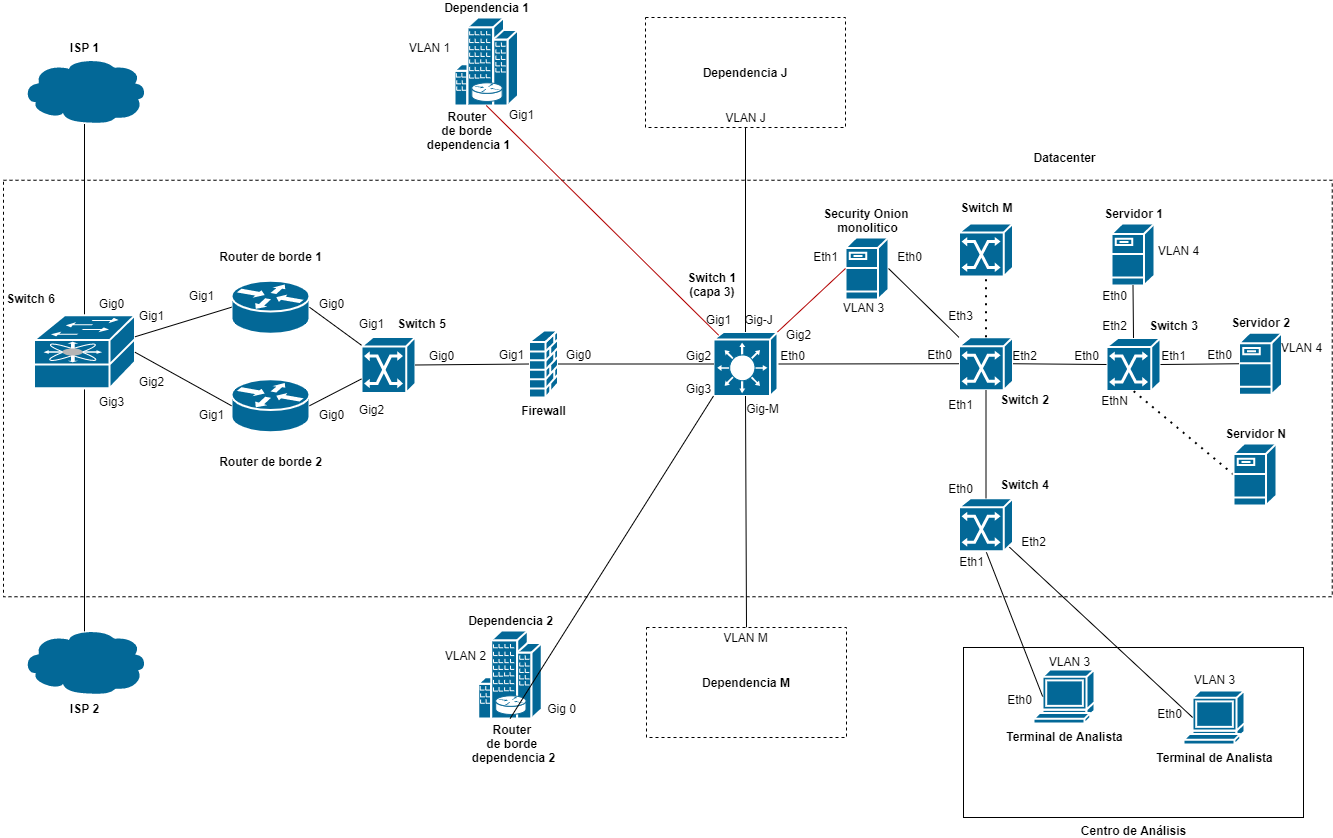
\includegraphics[width=1\textwidth]{./iteracion_1_imagenes/figura_topologia_m_unc.png}
    \caption{Despliegue de una topología monolítica de monitoreo}
    \label{fig:iter1_top_m_unc}
    \end{figure}
    \FloatBarrier
    Se realizaron pruebas de los requerimientos funcionales 1 y 3: se comprobó el funcionamiento de la recolección y almacenamiento de datos de incidentes de seguridad, al recibir y analizar tráfico proveniente de la Dependencia 1. \par
    %El nodo monolítico de Security Onion dispone de dos conexiones. La correspondiente al puerto eth0 es la que permite la administración del sistema y la consulta de sus datos, mientras que la interfaz eth1 es la destina a monitorear el tráfico de una red. En nuestro experimento con esta arquitectura, todo el tráfico fue simulado usando los PCAPS mencionados anteriormente. \par
    %En la Figura \ref{fig:iter1_top_m_unc} se observa la topología de la organización con un nodo Monolítico. Este tiene su interfaz de monitoreo conectada al Switch 3, donde recibe el tráfico reenviado que se produce entre la Dependencia 1 y el mencionado switch.
    
    \end{subsection}
    
    \begin{subsection}{Topología Distribuida de Monitoreo}
    \label{sec_topo_dist}
    Después de comprobar el funcionamiento de los principales componentes de Security Onion y obtener la experiencia descrita en la sección anterior, se procedió a considerar el despliegue de una topología distribuida. Este tipo de topología presenta considerables ventajas respecto de su alternativa monolítica, fundamentalmente en términos de rendimiento del hardware y flexibilidad de adaptación, como se mencionó en el Capítulo 4.\par
    En primer lugar, se desplegó una versión simplificada para verificar el funcionamiento de los componentes de los dos nodos que la componen (nodos \textit{Forward} y \textit{Master}) y la comunicación entre ellos.
    \begin{figure}[H]
    \centering
    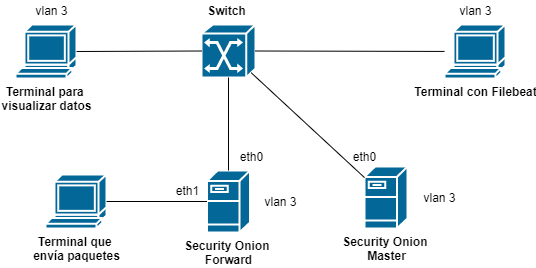
\includegraphics[width=1\textwidth]{./iteracion_1_imagenes/figura_33_b_topologia_de_prueba_2.png}
    \caption{Versión elemental de una topología distribuida}
    \label{fig:topologia_distribuida_1}
    \end{figure}
    Se observa en la Figura \ref{fig:topologia_distribuida_1} los componentes fundamentales de Security Onion para poder llevar a cabo esta topología: un nodo \textit{Forward} conectado a la interfaz a monitorear y un nodo \textit{Master} conectado al switch de la red interna. El nodo \textit{Master} y el \textit{Forward} se comunican mediante un enlace de administración (interfaz eth0 del nodo \textit{Forward}), que es el que está conectado al Switch. \par
    En este caso, como en el descrito en la sección anterior (\ref{subsec-topo-mono}), se utilizaron logs y tráficos de red obtenidos con anterioridad. El objetivo de esta experiencia fue comprobar el correcto funcionamiento de los dos nodos. Adicionalmente, con el motivo de probar la generación de notificaciones de alertas, se comprobó el funcionamiento de ElastAlert, que forma parte de los componentes del nodo \textit{Master}. \par
    La experiencia consistió en enviar logs desde la terminal con Filebeat hacia el nodo \textit{Master}, para que posteriormente fueran filtrados. Para esta tarea se empleó Logstash junto a un \textit{plugin} llamado Grok. Se buscó identificar campos de interés que estuvieran presentes en los \textit{logs} y se hallaron direcciones IP. Se crearon alertas en ElastAlert que se activaron al detectar estas IP y se enviaron mensajes por un servidor de correo electrónico (propio de la organización) y aplicaciones (Telegram y Slack). Los resultados de este experimento verificaron el RF4, que se trata en la iteración II (Capítulo \ref{iteracion2}). \par
    Si bien Security Onion incluye gran parte de los componentes de un SIEM, es necesario un sistema adicional que sea capaz de recolectar las alertas generadas en primera instancia por el nodo \textit{Master} y manipular esta información para lograr un manejo eficaz de los incidentes. Este sistema es TheHive. \par
    TheHive recibe las alertas generadas en el nodo \textit{Master} por ElastAlert y las introduce en un proceso de correlación de incidentes para proporcionar mayor información del mismo a los analistas del CSIRT. Cortex es un componente asociado a TheHive, que permite desarrollar y automatizar respuestas a incidentes. TheHive y Cortex, junto a los componentes del nodo \textit{Master} (Kibana y Squert) son los únicos componentes visibles con los que interactúan los analistas. \par
    
    Luego de la incorporación de TheHive, se volvió a repetir el experimento detallado anteriormente (Figura \ref{fig:topologia_distribuida_1}), esta vez con el objetivo de que TheHive recibiera las alertas generadas en el nodo \textit{Master} mediante ElastAlert. La topología del experimento se observa en la Figura \ref{fig:topologia_distribuida_2}.\par
    \begin{figure}[H]
    \centering         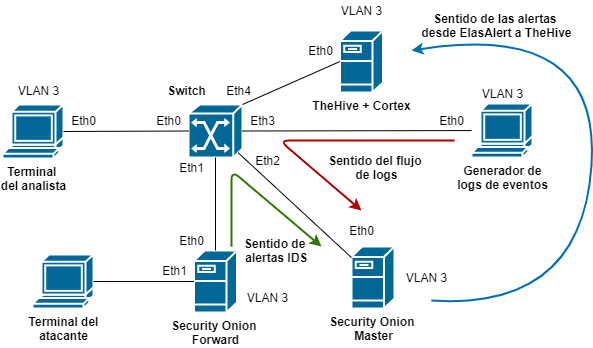
\includegraphics[width=1\textwidth]{./iteracion_1_imagenes/figura_33_e_topologia_de_prueba_3.png}
    \caption{Experiencia de laboratorio de la topología distribuida con todos sus componentes}
    \label{fig:topologia_distribuida_2}
    \end{figure}
    \FloatBarrier
    De esta manera, se completaron los componentes del SIEM al ofrecer un manejo centralizado de los datos de incidentes de seguridad de la información. Cuando el nodo \textit{Forward} identificó un  ataque, notificó al nodo \textit{Master} del mismo. En este último, ElastAlert generó alertas que fueron enviadas al servidor de TheHive, quien las presentó a los analistas junto a información contextual que intentó correlacionar con información presente en su base de datos.\par
    
    Finalmente, se procedió a desplegar la configuración final de la topología de la solución en este proyecto. Esta consistió en agregar un segundo nodo \textit{Forward} para monitorear el tráfico de una dependencia adicional, como se muestra en la Figura \ref{fig:iter1_top_d_unc}.
    \begin{figure}[H]
    \centering
    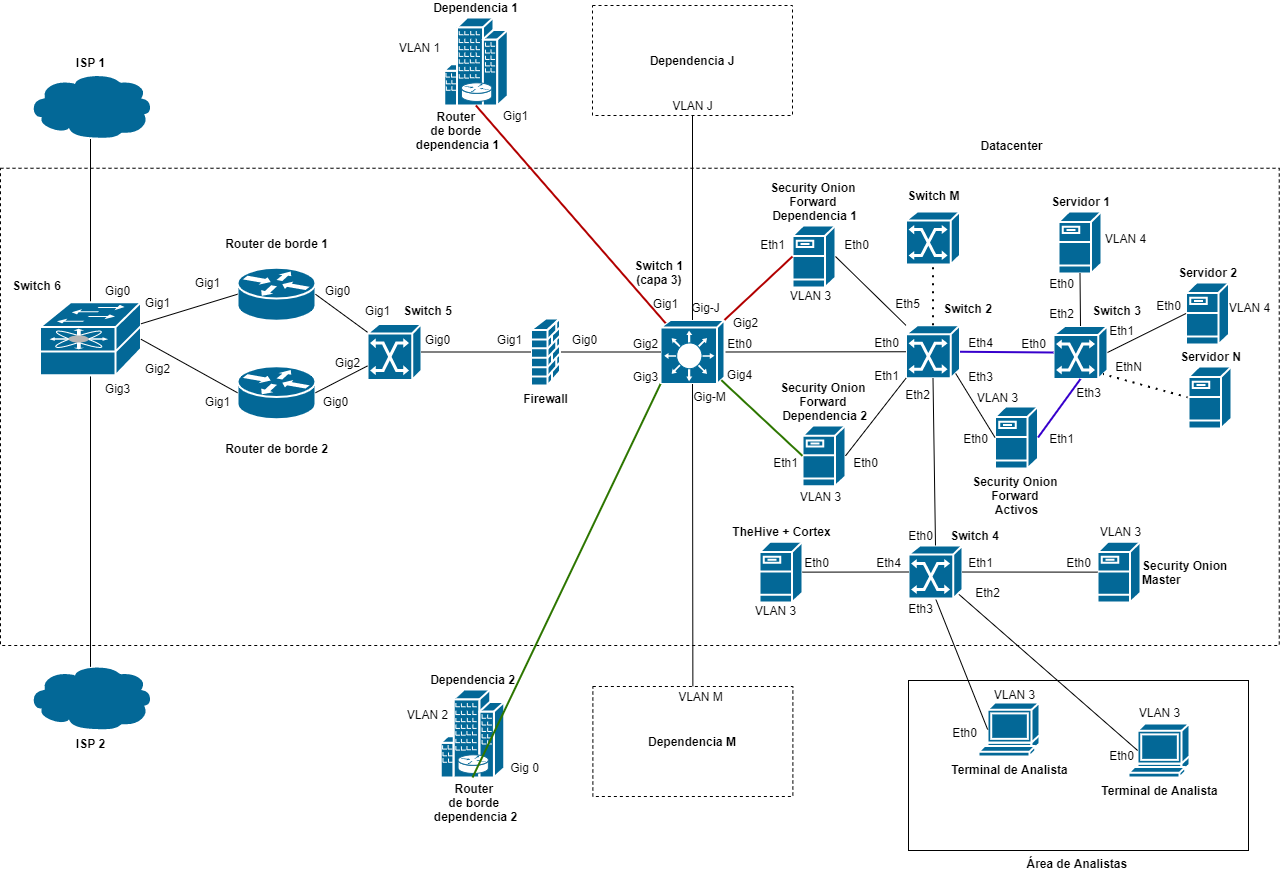
\includegraphics[width=1\textwidth]{./iteracion_1_imagenes/figura_topologia_d_unc.png}
    \caption{Despliegue de una topología distribuida de monitoreo}
    \label{fig:iter1_top_d_unc}
    \end{figure}
    La Figura \ref{fig:iter1_top_d_unc} muestra la topología de prueba donde se instaló Security Onion. Se observan los proveedores de conexión a internet (ISP) y la conexión con el \textit{router} de borde de la organización. Este último se conecta mediante un enlace \textit{gigabit} en el puerto Gig0 al puerto Gig4 del \textit{Switch} 1 (capa 3). \par
    El \textit{Switch} 1 es un dispositivo de red de capa 3, que conecta las dependencias entre sí y con el \textit{datacenter}. Las conexiones mencionadas se implementan físicamente sobre un enlace \textit{gigabit} de fibra óptica, pero virtualmente sobre redes tipo VLAN. De esta manera, por ejemplo, la Dependencia 1 está conectada físicamente por un enlace \textit{gigabit} a través de su puerto Gig1 de su \textit{router} de borde, con el puerto Gig5 del Switch 1 capa 3. Desde el punto de vista lógico, este enlace pertenece a la VLAN 1 de la organización. La situación descrita es análoga para el resto de las dependencias de la Universidad. \par
    Por otro lado, el \textit{Switch} 1 (en adelante SW 1), está conectado a los nodos \textit{Forward} 1 y 2 de Security Onion. Como resultado, es posible reenviar el tráfico entre SW1 y las dependencias 1 y 2 hacia los puertos Gig0 y Gig2 de SW1 que conectan SW1 con los nodos \textit{Forward} 1 y 2. \par
    SW1 está conectado con el \textit{Switch} 2 perteneciente al \textit{datacenter}, al cual se conectan a su vez los terminales de los analistas, los nodos \textit{Master} y \textit{Forward} (1 y 2) de Security Onion y TheHive. Esta topología permite desplegar una arquitectura distribuida de Security Onion, que fue la elegida para este proyecto.
    \end{subsection}
    \begin{section}{Verificación de RF1 y RF3}
    Luego de haber desplegado la topología distribuida que se observa de la Figura \ref{fig:iter1_ver_RF1_RF2}, se verificó el cumplimiento de los requerimientos RF1 y RF3. Para ello se llevó a cabo una acción ofensiva sobre un servidor ubicado en el \textit{datacenter}. Se seleccionó este servidor mediante un acuerdo con los responsables del área, para fines de evaluación de este proyecto. Este activo de la organización fue configurado a modo de prueba con un servidor web Apache versión 2.4.46, que contaba con una formulario web en PHP versión  7.2.21  y una base de datos MySQL versión 8.0.17.\par
    \begin{figure}[H]
    \centering
    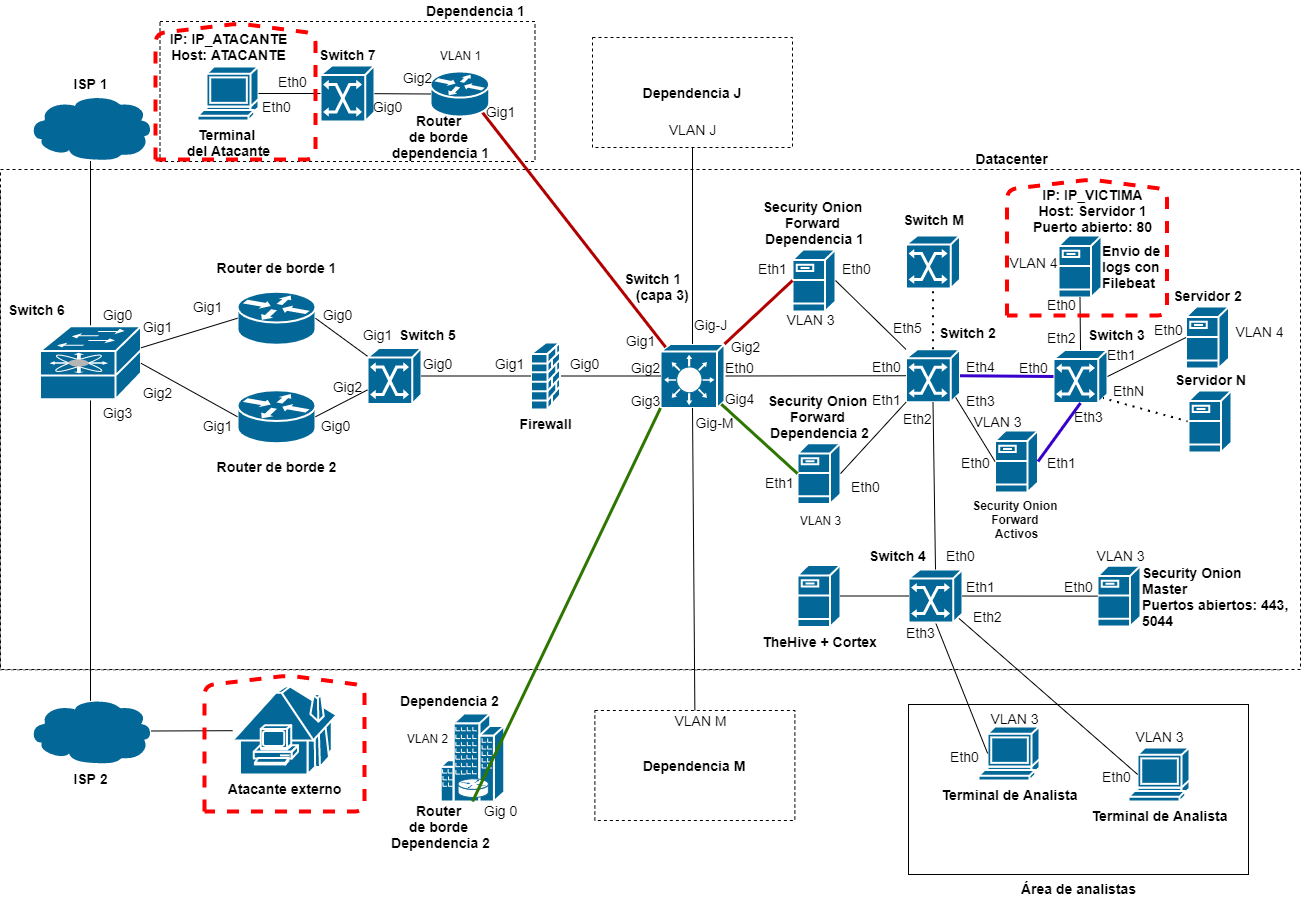
\includegraphics[width=1\textwidth]{./iteracion_1_imagenes/Topologia de despliegue descentralizada RF2, RF6 y RF4.png}
    \caption{Despliegue de una topología distribuida de monitoreo}
    \label{fig:iter1_ver_RF1_RF2}
    \end{figure}
    La acción ofensiva consistió en un ataque de reconocimiento que partió desde el \textit{host} ATACANTE ubicado dentro de la Dependencia 1 hacia la víctima llamada Servidor 1 que se encontraba dentro del \textit{datacenter}.
    Para realizar el ataque de reconocimiento se utilizaron rutinas de NMAP \cite{nmap} (versión 7.80) configuradas a tal fin: \textit{nmap -T4 -A -v IP\_VICTIMA} . Los parámetros utilizados fueron:
    \begin{itemize}
    \item -T4: para un escaneo intensivo (disminuye el tiempo de ejecución entre \textit{scripts})
    \item -A: habilita la detección del sistema operativo de la víctima y su versión, los \textit{scripts} de escaneo y \textit{traceroute}.
    \item -v: habilita el modo “verboso”.
    \item IP\_VICTIMA: es la dirección IP objetivo de este reconocimiento.
    \end{itemize}
    En la Figura \ref{fig:squert-nmap} se observa el panel de visualización de eventos de Squert.  En el recuadro rojo se encuentra la detección del ataque de reconocimiento realizado. El resto de la información que se aprecia en el panel principal corresponde a otros eventos que el sistema estaba detectando. Los eventos se agrupan según la categoría a la que pertenecen y un indicador de colores (barra vertical a la derecha del contador de eventos de cada fila) indica su prioridad de atención. %*Por defecto, Squert tiene su propia categoría de prioridades.
    Luego se observan la cantidad de eventos según su dirección, hora del último incidente ocurrido junto con su ID, una descripción de la firma del evento y el porcentaje de ocurrencia respecto al total de incidentes detectados.
    \begin{figure}[H]
    \centering
    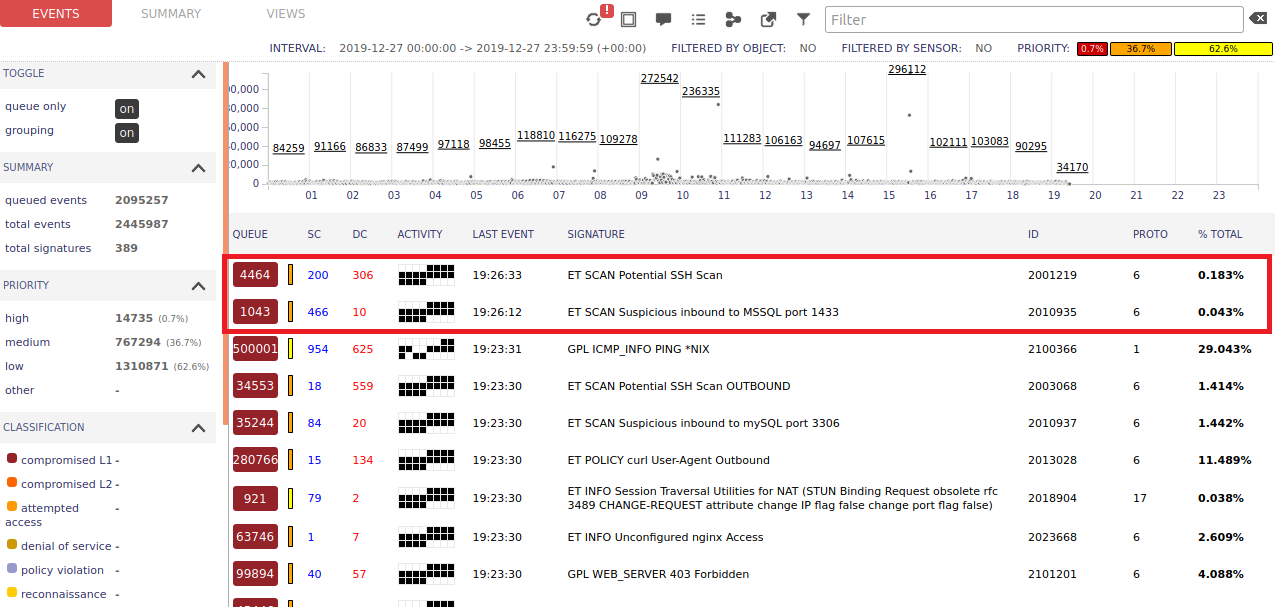
\includegraphics[width=1\textwidth]{./iteracion_1_imagenes/Squert_NMAP.png}
    \caption{Eventos visualizados en Squert}
    \label{fig:squert-nmap}
    \end{figure}
    \FloatBarrier
    En la Figura \ref{fig:thehive-nmap} se observa la visualización de la detección en TheHive. Si bien pueden ser similares, Squert se limita a mostrar los ataques similares agrupados en la misma categoría de incidente al que pertenecen, mientras que TheHive recibe las alertas de ElastAlert y presenta los eventos de manera individual. Esto permite a los analistas crear casos con cada incidente, correlacionarse con otros ataques, etc, lo que conduce a una gestión integral de eventos de seguridad.
    \begin{figure}[H]
    \centering
    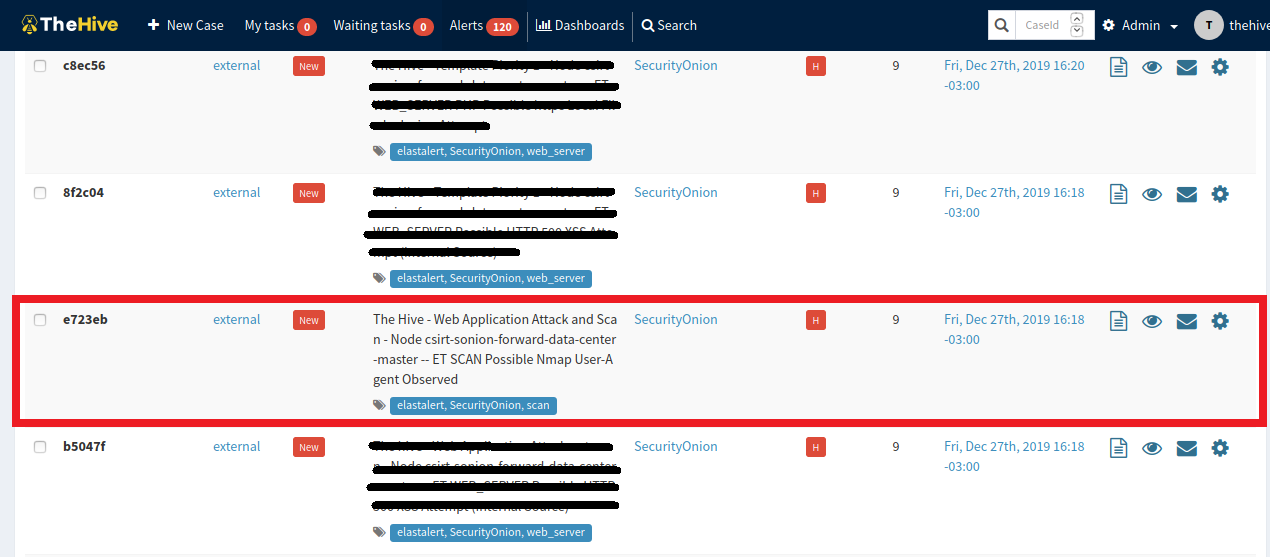
\includegraphics[width=1\textwidth]{./iteracion_1_imagenes/TheHive-NMAPEditado.png}
    \caption{Detección en TheHive del ataque de reconocimiento}
    \label{fig:thehive-nmap}
    \end{figure}
    \FloatBarrier
    Se verificó que las direcciones IP reportadas en el incidente por Squert y TheHive, coincidieran con las de la víctima y el atacante. Además mientras se estaba ejecutando el ataque, se hizo un seguimiento mediante Wireshark \cite{wireshark} filtrando las direcciones IP de origen y destino. Esto permitió corroborar el flujo de datos entre ambos.
    Los ataques fueron detectados por los nodos \textit{Forward} de la Dependencia 1 y \textit{Forward} Activos. \par
    Con esta prueba se verifica el cumplimiento de los requerimientos funcionales 1 y 3: “recolectar y almacenar datos de incidentes de seguridad en la infraestructura de la red corporativa ” y “visualizar las alertas en un tablero de mando”.\par
    \end{section} 
    
    
    \begin{section}{Colorario}
    En cuanto a la topología de la organización (Figura \ref{fig:iter1_top_unc}), podemos concluir que, la mejor opción para monitorear el tráfico entre las dependencias de la organización y el exterior fue conectar los nodos \textit{Forward} al \textit{Switch} 1 (el \textit{switch} troncal), para recibir el tráfico reenviado entre las dependencias y el mencionado \textit{switch}. Por otro lado, con el objetivo de lograr una defensa de punto final sobre activos de información específicos, fue necesario conectar un nodo \textit{Forward} al \textit{switch} (\textit{Switch} 2) al que se encuentran conectados estos activos. Estas conexiones se vieron reflejadas en la Figura \ref{fig:iter1_ver_RF1_RF2}. \par
    Se observó que la topología Monolítica fue ineficiente para el uso en entornos de producción, dado que la pila Elastic y los componentes de los sensores IDS de este nodo demandaron un uso intensivo de \textit{hardware}. Si bien este tipo de topología fue útil a fines de probar el sistema o para monitorear enlaces de reducido tráfico y poco ancho de banda, resultó ineficaz en entornos más complejos. Esto se debió a los enormes requisitos de hardware necesarios para monitorear un enlace de 1 Gbps y considerando que el despliegue final requirió el monitoreo de múltiples enlaces con este ancho de banda, este tipo de topología fue incapaz de escalar utilizando el hardware disponible.\par
    Como consecuencia de la incapacidad de escalamiento horizontal descrita y siendo esta un requerimiento no funcional de este proyecto, se desplegó una topología distribuida de Security Onion. Los resultados del monitoreo fueron positivos, por lo cual se dio cumplimiento al RNF3, en simultáneo con la verificación de RF1 y RF3.\par
    

    \end{section}